%========================================
% UniLearn Hub - Report
%========================================
\documentclass[12pt,a4paper]{article}

%---------- Packages ----------
\usepackage[margin=2.5cm]{geometry}
\usepackage{setspace}
\usepackage{parskip}
\usepackage{graphicx}
\usepackage{booktabs}
\usepackage{array}
\usepackage{titlesec}
\usepackage{hyperref}
\usepackage{xcolor}
\usepackage{fancyhdr}
\usepackage{caption}
\usepackage{float}
\usepackage{tabularx}
\usepackage{longtable}
\usepackage{listings}
\usepackage{seqsplit}
\usepackage[utf8]{inputenc}
\usepackage[T1]{fontenc}
\usepackage{tgschola}

\newcolumntype{Y}{>{\raggedright\arraybackslash}X}

%---------- Basic formatting ----------
\onehalfspacing

\hypersetup{
    colorlinks=true,
    linkcolor=black,
    urlcolor=blue!60!black,
    citecolor=black,
    pdfauthor={Syed Imad Uddin},
    pdftitle={WM243-18 IM CW1}
}

%---------- Colour and section styles ----------
\definecolor{warwickpurple}{RGB}{87, 35, 100}

\titleformat{\section}
  {\large\bfseries\color{warwickpurple}}
  {\thesection}{1em}{}

\titleformat{\subsection}
  {\normalsize\bfseries}
  {\thesubsection}{0.75em}{}

\titleformat{\subsubsection}
  {\normalsize\itshape}
  {\thesubsubsection}{0.75em}{}

%---------- Code listing style ----------
\lstset{
    basicstyle=\ttfamily\small,
    keywordstyle=\bfseries\color{warwickpurple},
    commentstyle=\itshape\color{gray},
    stringstyle=\color{blue!60!black},
    breaklines=true,
    frame=single,
    framerule=0.4pt,
    rulecolor=\color{gray!40},
    backgroundcolor=\color{gray!5},
    numbers=none,
    showstringspaces=false,
    tabsize=4,
    xleftmargin=0.5cm,
    xrightmargin=0.5cm,
    aboveskip=0.8em,
    belowskip=0.8em
}

%---------- Header and footer ----------
\pagestyle{fancy}
\setlength{\headheight}{14pt}
\fancyhf{}
\lhead{\small WM243-18 IM CW1}
\rhead{\small UniLearn Hub}
\cfoot{\small \thepage}

%========================================
\begin{document}

%---------- Title Page ----------
\begin{titlepage}
    \thispagestyle{empty}
    \centering
    \vspace*{1.5cm}

    
\includegraphics[width=0.55\textwidth]{images/u_of_w_third_party_lockup_positive_rgb.jpg}\\[1.5cm]

    {\Large \textbf{WM243-18 IM CW1}}\\[0.5cm]
    {\large UniLearn Hub}\\[0.3cm]
    {\large Report}\\[2cm]

    {\large Information Management Coursework}\\[2cm]

    \vfill

    {\large \textbf{Student:} Syed Imad Uddin}\\[0.5cm]
    {\large \today}

    \vfill
\end{titlepage}

%---------- Table of Contents ----------
\tableofcontents
\newpage

%========================================
\section{Design and Export a Secure PostgreSQL Database Schema}
\label{sec:task1}
%========================================

\subsection{ERD}
\label{sec:erd}

The diagram below is the Crow's Foot entity relationship diagram for the schema, covering all 16 tables and their foreign key relationships, including the zero or one cardinality on the nullable \lstinline|Notifications| and \lstinline|Messages| foreign keys.

\begin{figure}[H]
\centering
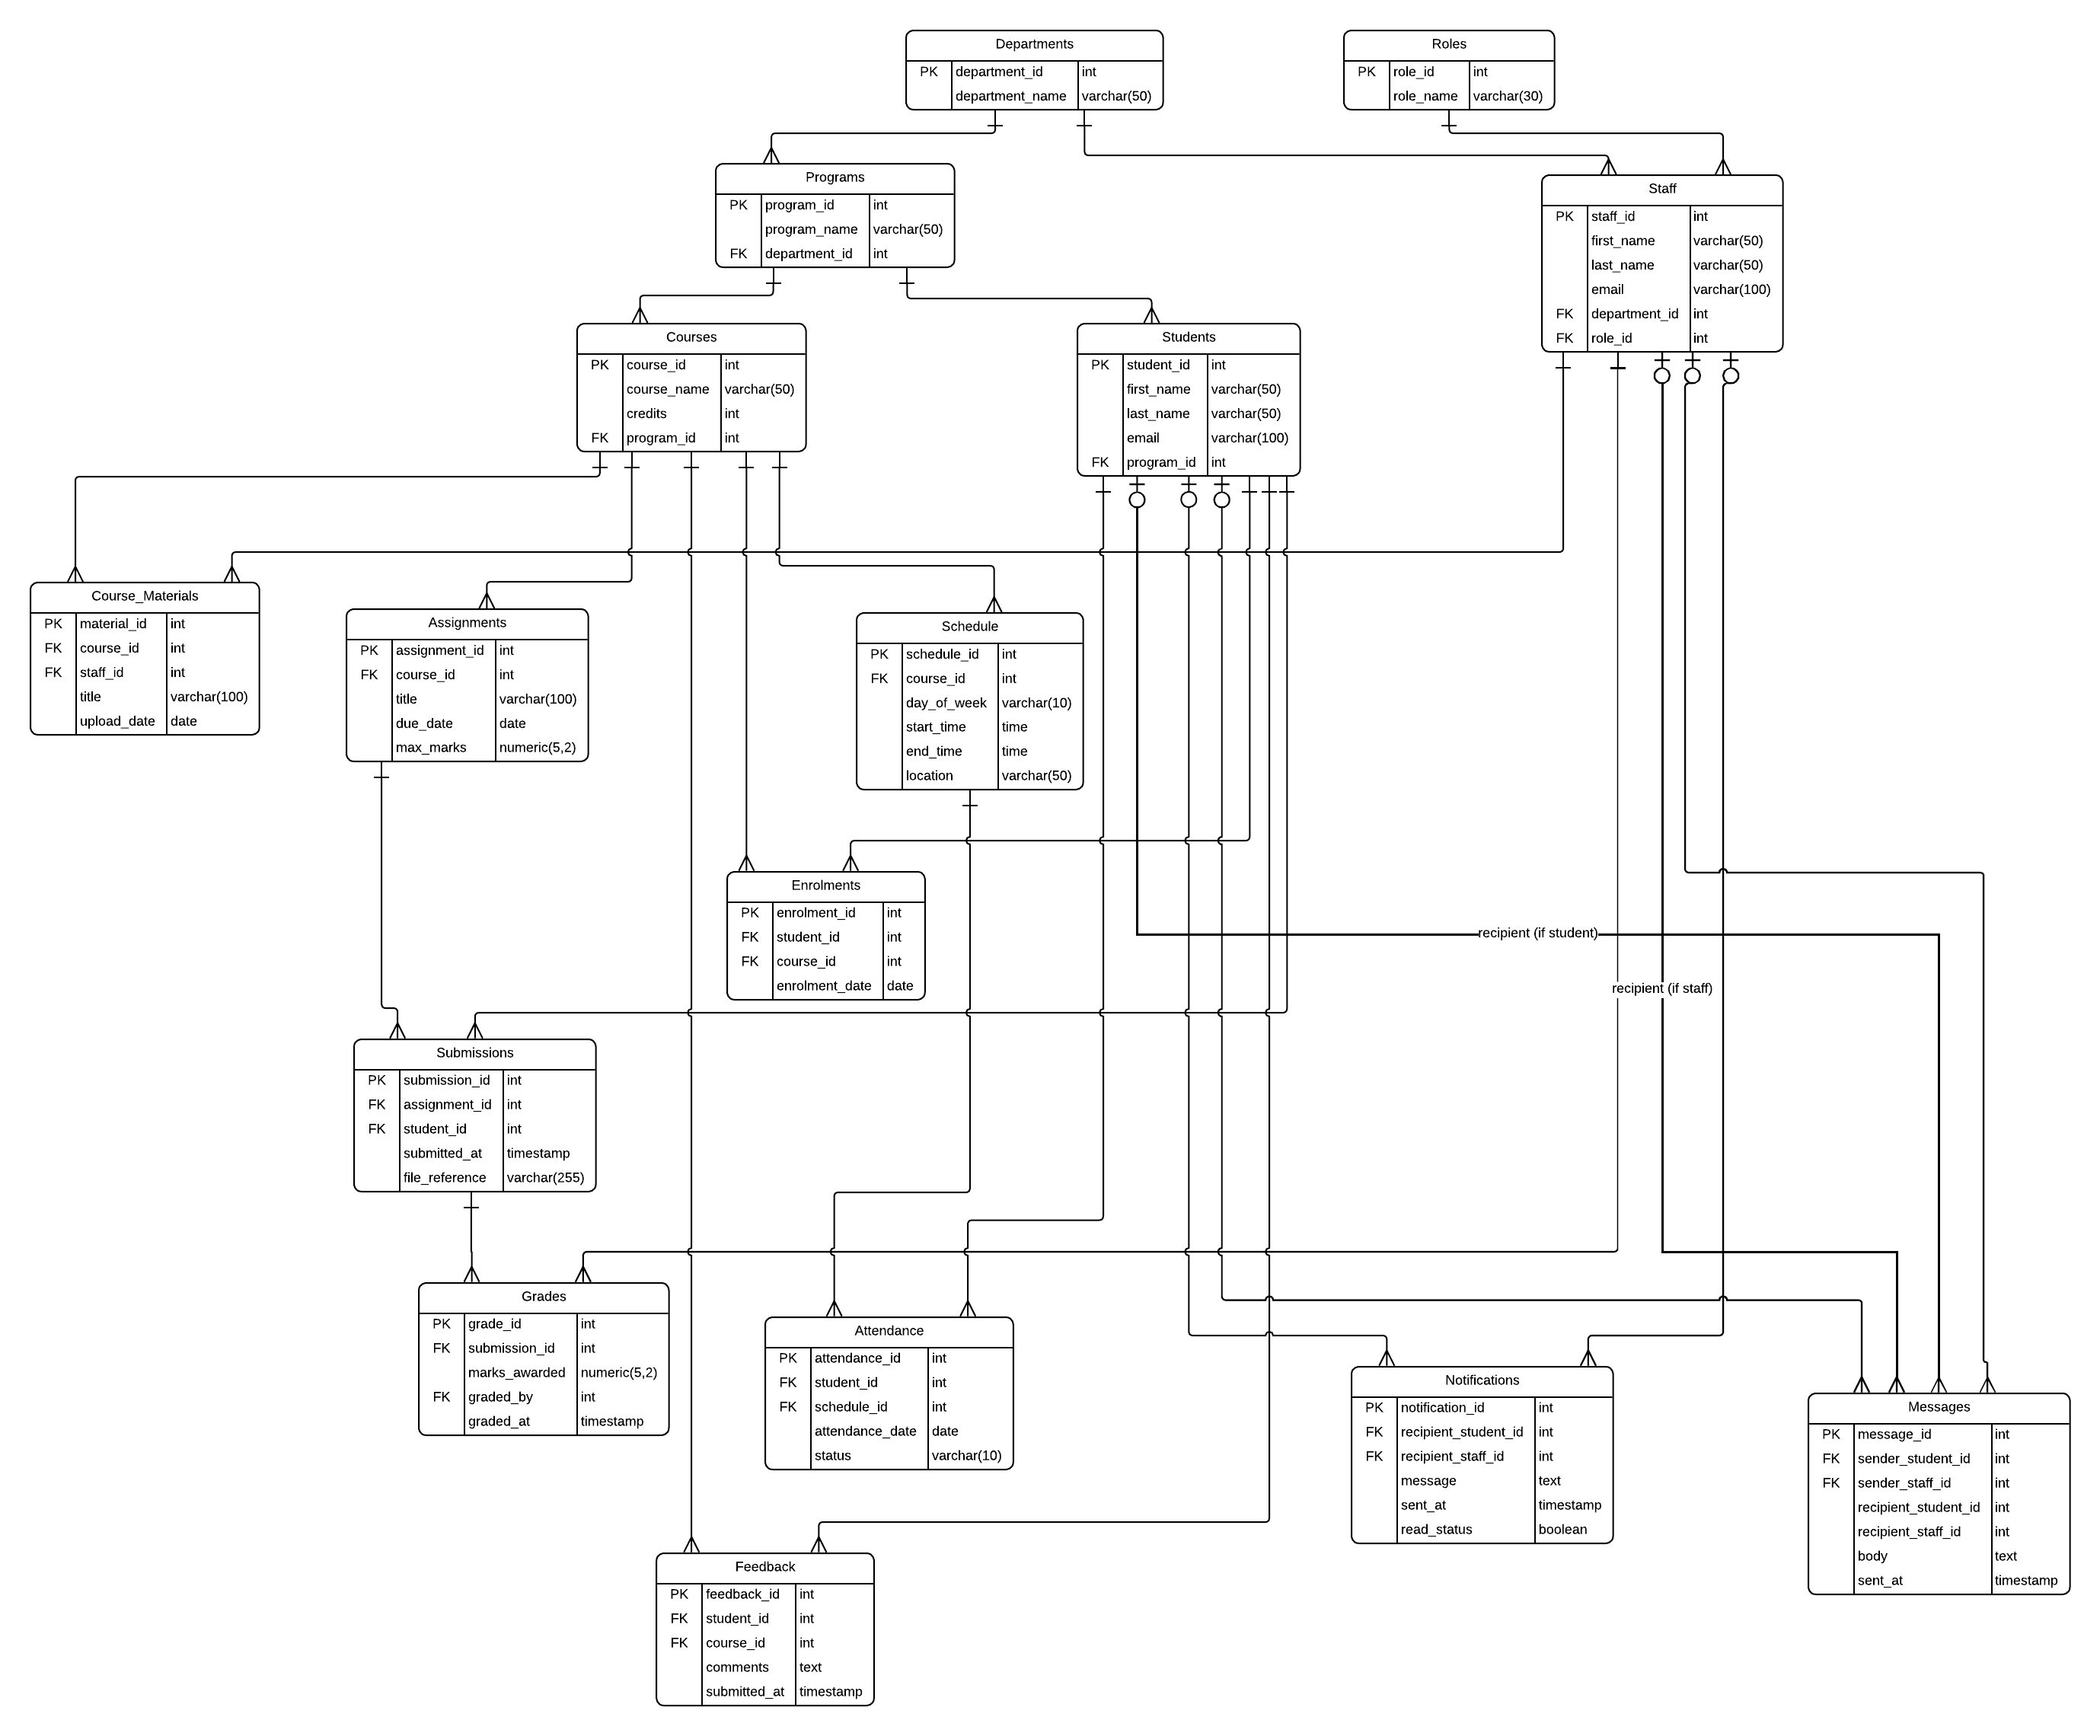
\includegraphics[width=\textwidth]{images/erd.png}
\caption{UniLearn Hub entity relationship diagram, Crow's Foot notation}
\end{figure}

\subsection{Entities and relationships}
\label{sec:entities}

I built the schema as 16 tables in a dedicated \lstinline|unilearn| schema, not \lstinline|public|, so the database can host other schemas alongside it without name collisions.

Four tables have no foreign keys and sit at the top of the dependency graph. \lstinline|Departments| and \lstinline|Roles| have no dependencies at all. \lstinline|Programs| depends on \lstinline|Departments|. \lstinline|Staff| depends on \lstinline|Departments| and \lstinline|Roles|. Everything else builds on top of \lstinline|Students| (depends on \lstinline|Programs|) and \lstinline|Courses| (depends on \lstinline|Programs|).

I resolved the many to many relationships with two junction tables, \lstinline|Enrolments| (student and course) and \lstinline|Submissions| (assignment and student). Each has a \lstinline|UNIQUE| constraint on the pair of foreign keys so the same relationship can't be inserted twice. \lstinline|Grades| sits one level further down, one to one with \lstinline|Submissions| through a \lstinline|UNIQUE NOT NULL| foreign key, so a submission has at most one grade.

\lstinline|Notifications| and \lstinline|Messages| model a recipient, and for \lstinline|Messages| a sender, that is either a student or a staff member, never both. I explain the constraint design behind this in Section~\ref{sec:normalisation}.

\lstinline|Course_Materials|, \lstinline|Assignments|, \lstinline|Schedule|, \lstinline|Attendance|, and \lstinline|Feedback| all hang off \lstinline|Courses| or \lstinline|Students|, recording the day to day activity the schema exists to track. I didn't store anything beyond what these features need. No scraped or inferred personal data, no column collecting more than the stated use case requires, in line with the brief's GDPR compliance expectation.

Every primary key is a plain \lstinline|INTEGER GENERATED ALWAYS AS IDENTITY| rather than a UUID, since this system has no need for multiple write nodes. A sequential key keeps joins smaller and easier to read at this scale, at the cost of row creation order being visible in the key, which I judged acceptable here.

Table screenshots below (\lstinline|schema.sql|), grouped by dependency layer.

\begin{figure}[H]
\centering
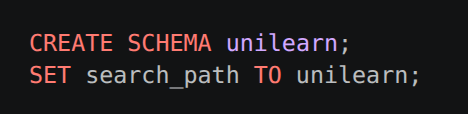
\includegraphics[width=0.6\textwidth]{images/01_schema_header.png}
\caption{Schema header}
\end{figure}

\begin{figure}[H]
\centering
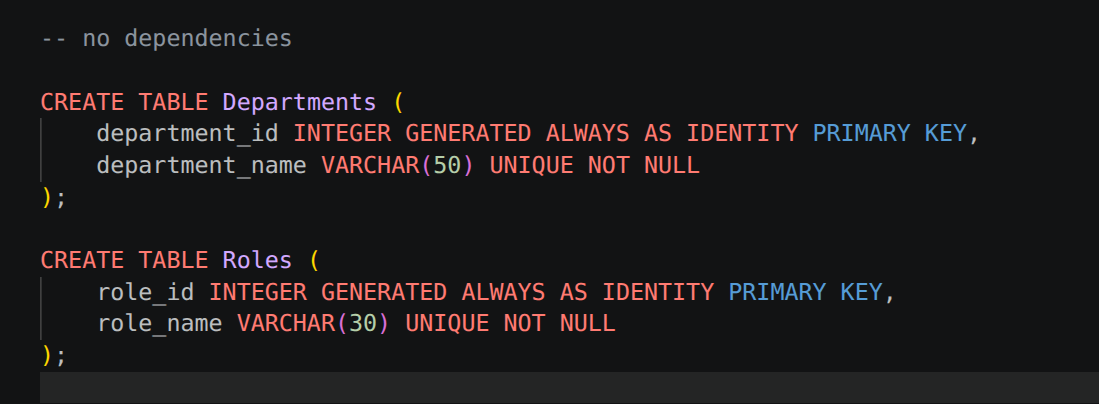
\includegraphics[width=0.75\textwidth]{images/02_departments_roles.png}
\caption{Departments, Roles}
\end{figure}

\begin{figure}[H]
\centering
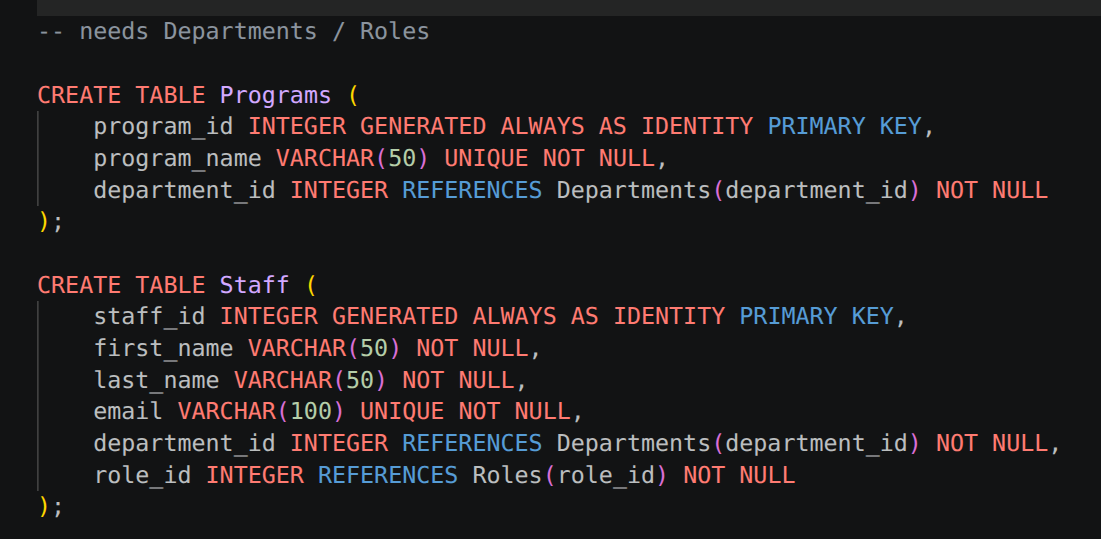
\includegraphics[width=0.85\textwidth]{images/03_programs_staff.png}
\caption{Programs, Staff}
\end{figure}

\begin{figure}[H]
\centering
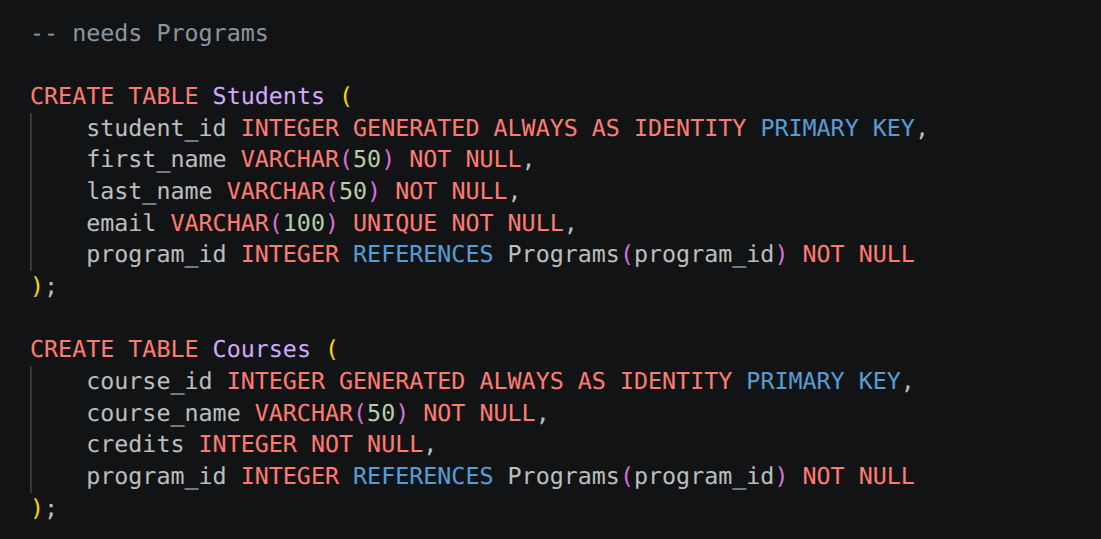
\includegraphics[width=0.85\textwidth]{images/04_students_courses.png}
\caption{Students, Courses}
\end{figure}

\begin{figure}[H]
\centering
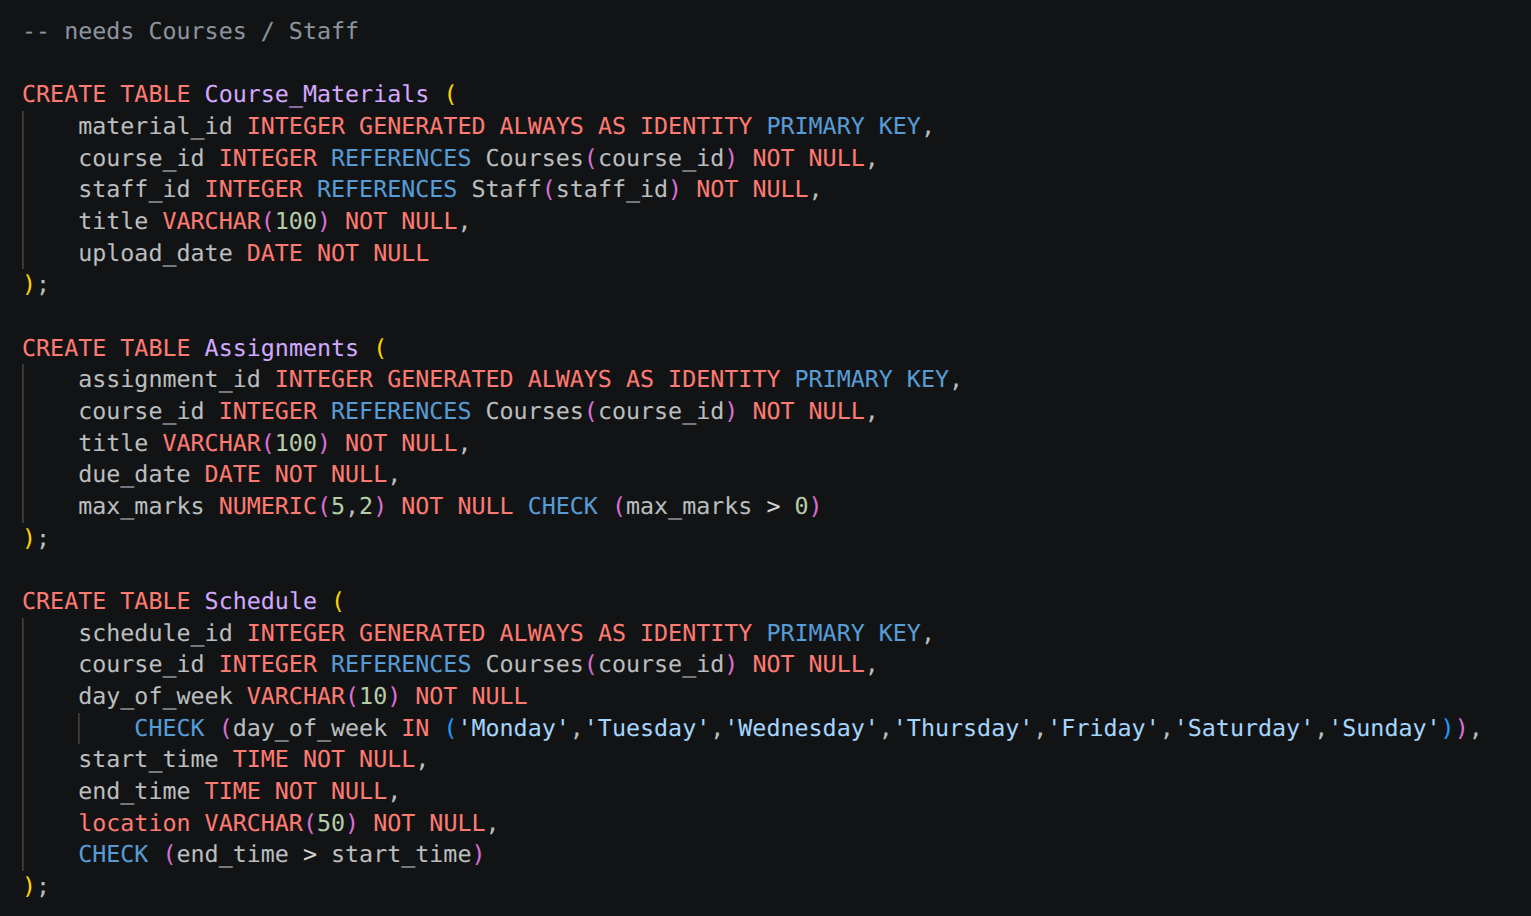
\includegraphics[width=\textwidth]{images/05_materials_assignments_schedule.png}
\caption{Course\_Materials, Assignments, Schedule}
\end{figure}

\begin{figure}[H]
\centering
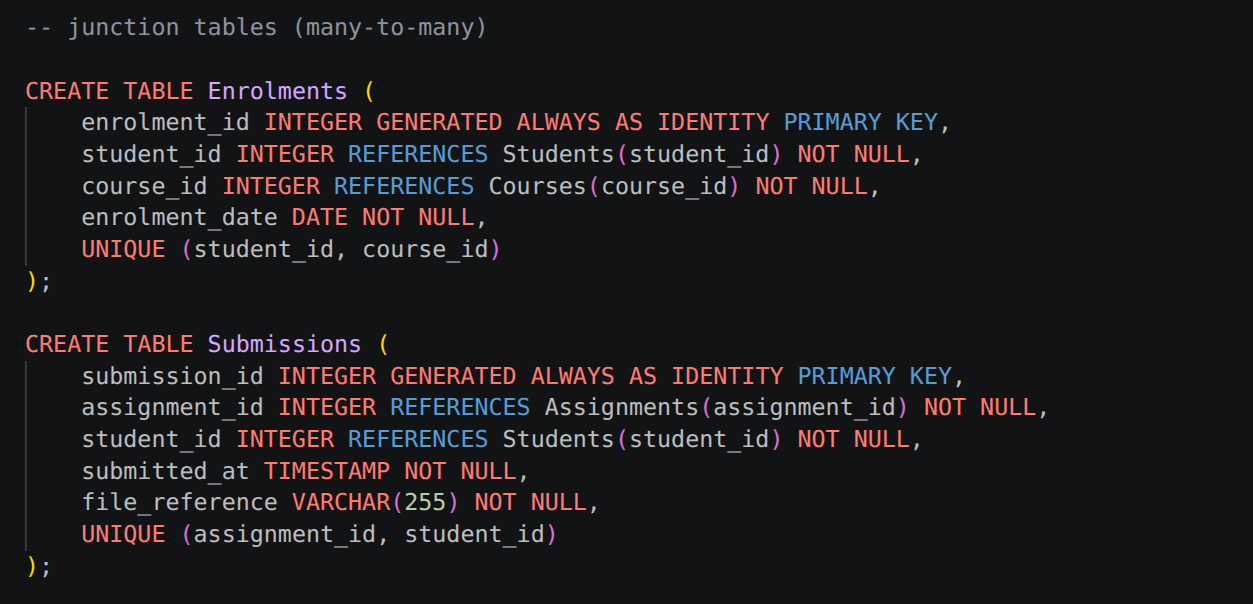
\includegraphics[width=0.9\textwidth]{images/06_enrolments_submissions.png}
\caption{Enrolments, Submissions}
\end{figure}

\begin{figure}[H]
\centering
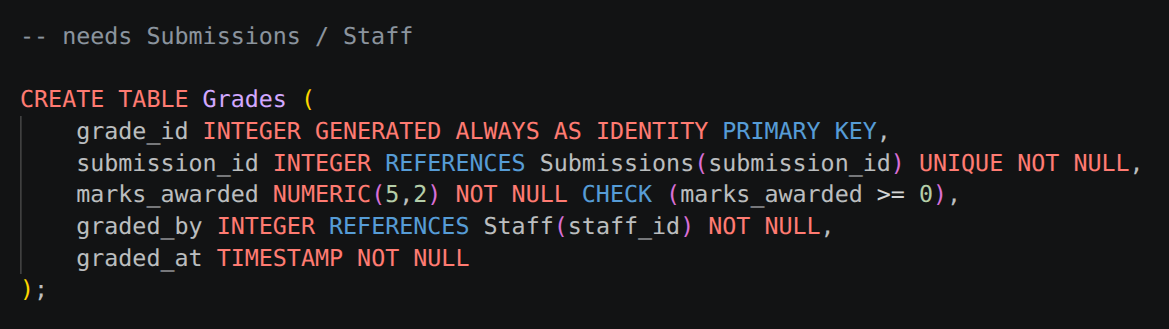
\includegraphics[width=0.7\textwidth]{images/07_grades.png}
\caption{Grades}
\end{figure}

\begin{figure}[H]
\centering
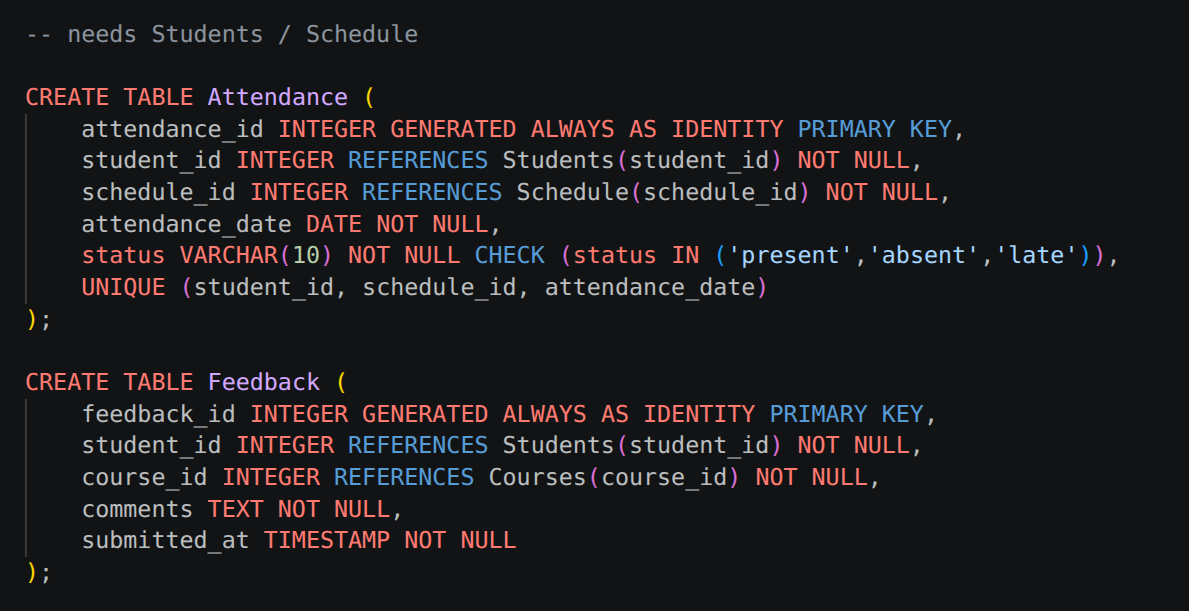
\includegraphics[width=0.85\textwidth]{images/08_attendance_feedback.png}
\caption{Attendance, Feedback}
\end{figure}

\begin{figure}[H]
\centering
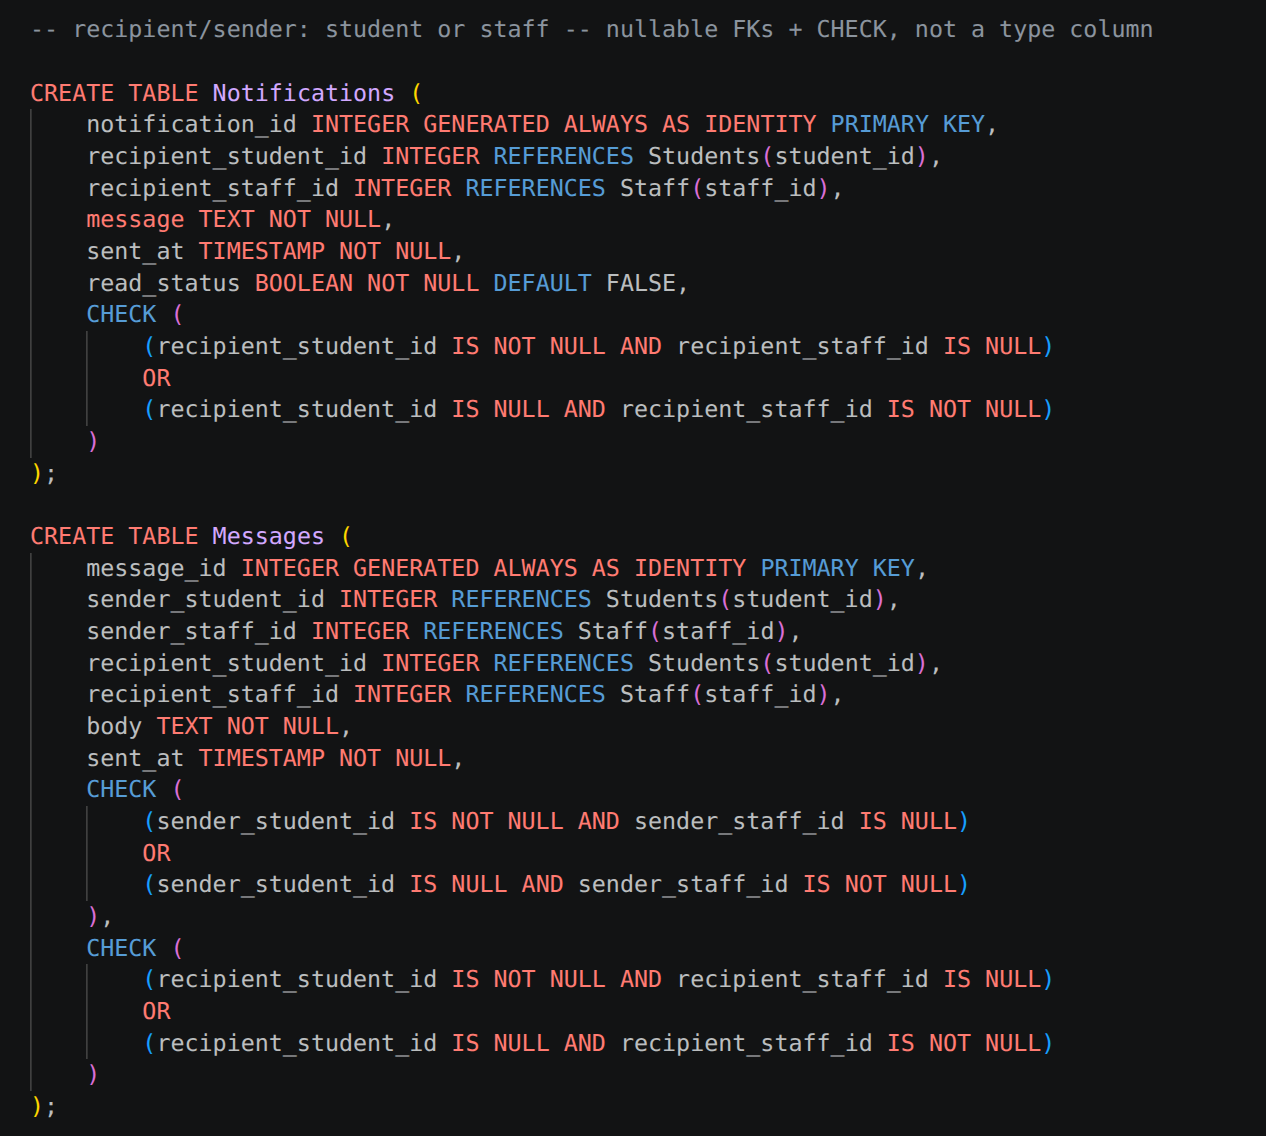
\includegraphics[width=\textwidth]{images/09_notifications_messages.png}
\caption{Notifications, Messages}
\end{figure}

\subsection{Normalisation and constraint design}
\label{sec:normalisation}

The schema is in 3NF. Every non key column depends on the whole primary key and nothing but the key. There is no repeating group data, a course's schedule is its own table, not a set of \lstinline|day1|, \lstinline|day2| columns, and no column is derivable from another column in the same row rather than stored directly.

\noindent\textbf{Junction tables over multi valued columns.} A student can enrol in many courses and a course has many students. Modelling this as an array column on either side would break 1NF and make listing every student in a course an unindexed scan. \lstinline|Enrolments| and \lstinline|Submissions| make both directions a plain indexed join, and their \lstinline|UNIQUE (a, b)| constraints double as the business rule that a student can't enrol in the same course twice.

\noindent\textbf{Nullable FK pair plus CHECK, not a subtype column.} \lstinline|Notifications| needed a recipient that is a student or a staff member. The alternative was a single \lstinline|recipient_type| column plus a \lstinline|recipient_id| with no foreign key at all, since one foreign key can't point at two different tables. That trades a real, database enforced foreign key for an application level convention with no constraint behind it. The \lstinline|CHECK| on the two nullable FKs rejects rows where both are null or both are set, at the database layer rather than the application layer. \lstinline|Messages| repeats the pattern for both sender and recipient.

\noindent\textbf{CHECK beyond NOT NULL.} \lstinline|Assignments.max_marks > 0|, \lstinline|Grades.marks_awarded >= 0|, \lstinline|Schedule.end_time > start_time|, and \lstinline|Attendance.status IN (...)| all encode a rule that is true for every valid row, so I put it in the schema rather than reimplementing it in every client that writes to these tables.

\noindent\textbf{Deliberately not built.} \lstinline|Grades.marks_awarded| has no \lstinline|CHECK| against its parent assignment's \lstinline|max_marks|. A \lstinline|CHECK| constraint can only see columns within its own row, so comparing against a different table needs a trigger. I left this out to keep the submitted schema fully trigger free and easy to reason about.

\subsection{Roles, grants, and views}
\label{sec:roles}

I exported four least privilege roles alongside the tables. \lstinline|admin_role| gets full access. \lstinline|lecturer_role| gets \lstinline|SELECT, INSERT, UPDATE| on the tables lecturers actively use, \lstinline|Courses|, \lstinline|Course_Materials|, \lstinline|Assignments|, \lstinline|Submissions|, \lstinline|Grades|, \lstinline|Feedback|, \lstinline|Schedule|, \lstinline|Attendance|, and \lstinline|SELECT| only on reference data, \lstinline|Students|, \lstinline|Enrolments|, \lstinline|Departments|, \lstinline|Programs|. That gives read access to the context they need and write access only to what they own. \lstinline|student_role| gets \lstinline|SELECT| on course facing tables, \lstinline|SELECT, INSERT| on \lstinline|Feedback|, and no grant at all on \lstinline|Grades|. \lstinline|read_only_role| gets \lstinline|SELECT| across the whole schema, for reporting and audit use.

I added two views to narrow what a role sees without exposing whole tables. \lstinline|Student_Grade_View| joins \lstinline|Submissions|, \lstinline|Assignments|, and \lstinline|Grades| but omits \lstinline|graded_by|, so a student sees their mark without seeing which staff member assigned it. \lstinline|Course_Roster_View| omits student email from the roster a lecturer sees. \lstinline|student_role| has no grant on \lstinline|Grades| itself, so the view is the only path to that data.

\begin{figure}[H]
\centering
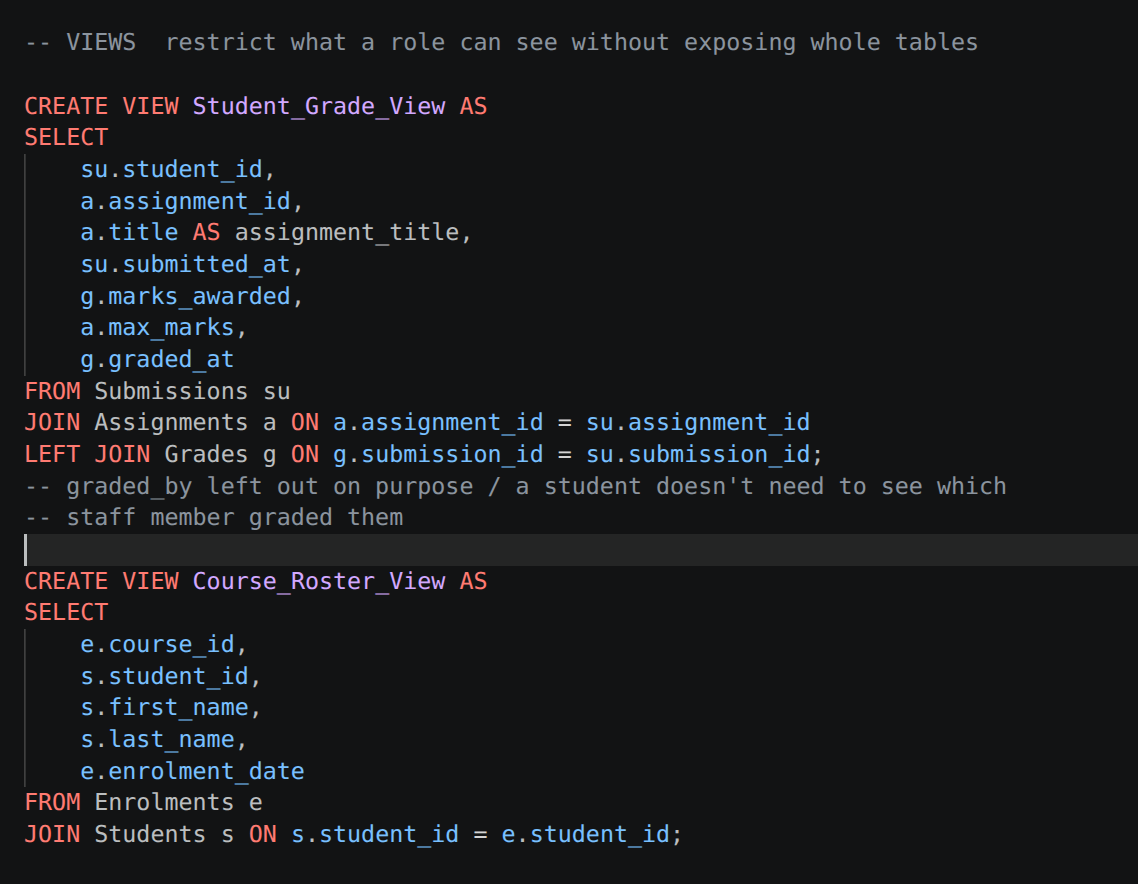
\includegraphics[width=0.75\textwidth]{images/10_views.png}
\caption{Student\_Grade\_View, Course\_Roster\_View}
\end{figure}

\begin{figure}[H]
\centering
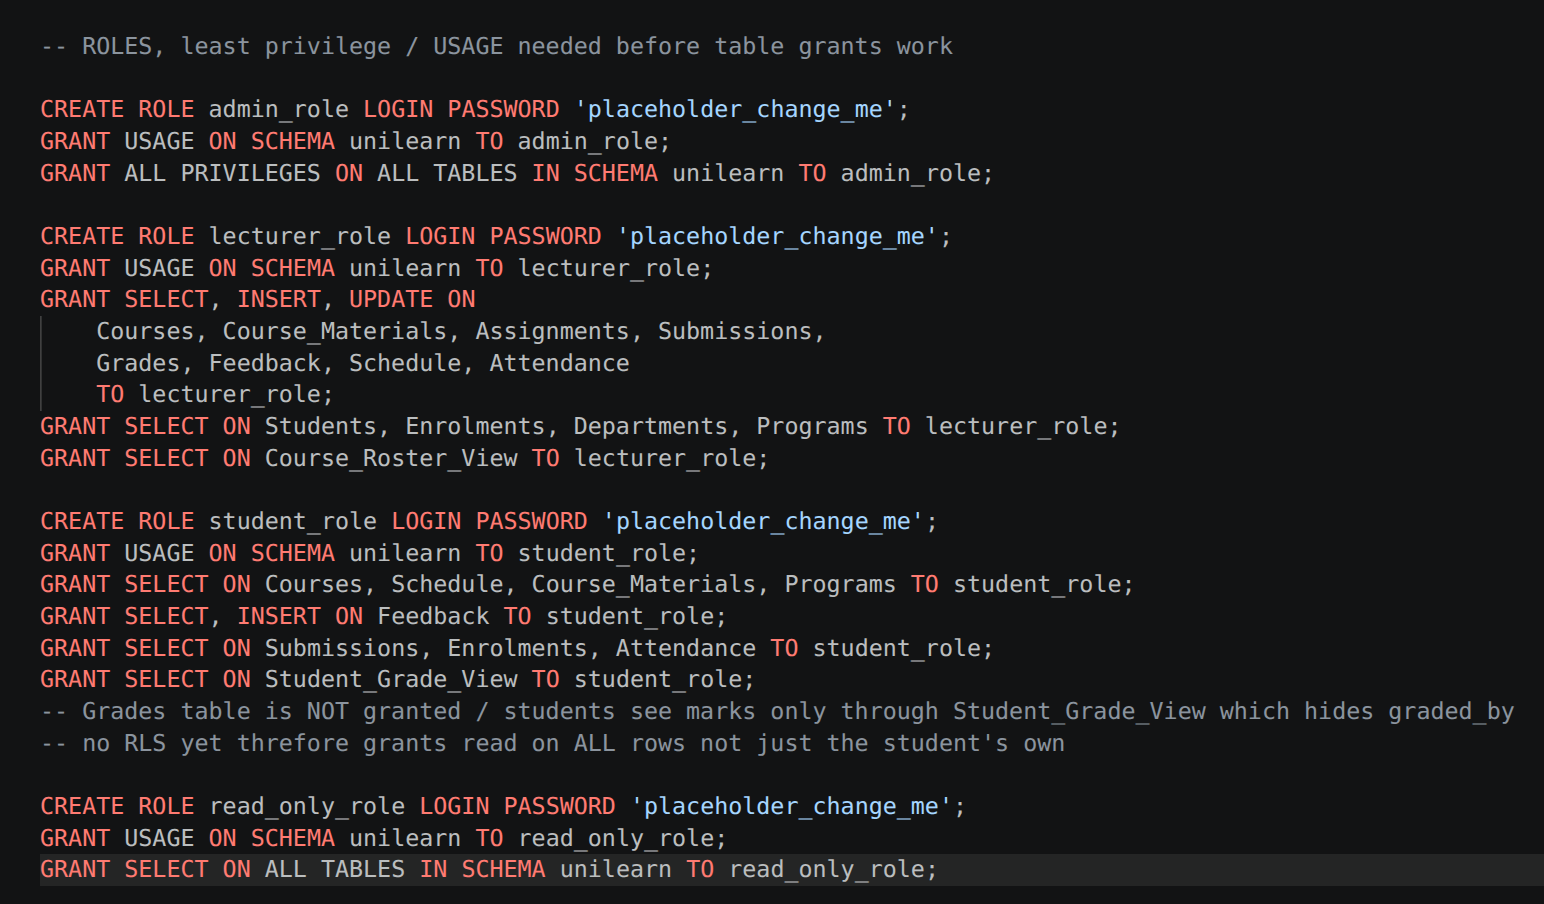
\includegraphics[width=0.85\textwidth]{images/11_roles_grants.png}
\caption{Roles and grants}
\end{figure}

\subsection{Verification}
\label{sec:verification1}

I tested this against a live PostgreSQL 18 instance rather than assuming it from the schema text. \lstinline|schema.sql| imported into a completely fresh database with zero errors, 16 \lstinline|CREATE TABLE|, 2 \lstinline|CREATE VIEW|, 4 \lstinline|CREATE ROLE| plus their grants.

\footnotesize
\renewcommand{\arraystretch}{1.3}
\begin{longtable}{@{} >{\raggedright\arraybackslash}p{3.2cm} >{\raggedright\arraybackslash}p{6.3cm} >{\raggedright\arraybackslash}p{5.5cm} @{}}
\caption{Schema, constraint, privilege, and view verification}\\
\toprule
\textbf{Test} & \textbf{Action} & \textbf{Result} \\
\midrule
\endfirsthead

\toprule
\textbf{Test} & \textbf{Action} & \textbf{Result} \\
\midrule
\endhead

\bottomrule
\endfoot

FK rejection & Insert an \lstinline|Enrolments| row referencing \lstinline|student_id = 999| (doesn't exist) & Rejected. \lstinline|violates foreign key constraint| \\[0.4em]
CHECK rejection & Insert a \lstinline|Notifications| row with both recipient FKs \lstinline|NULL| & Rejected. \lstinline|violates check constraint| \\[0.4em]
CHECK rejection & Insert a \lstinline|Notifications| row with both recipient FKs set & Rejected. Same constraint \\[0.4em]
CHECK acceptance & Insert a \lstinline|Notifications| row with exactly one recipient FK set & Succeeds \\[0.4em]
UNIQUE rejection & Insert a duplicate \lstinline|(student_id, course_id)| into \lstinline|Enrolments| & Rejected. \lstinline|violates unique constraint| \\[0.4em]
Privilege & \lstinline|lecturer_role|. \lstinline|SELECT| on \lstinline|Departments| & Succeeds. Granted explicitly \\[0.4em]
Privilege & \lstinline|lecturer_role|. \lstinline|INSERT|/\lstinline|UPDATE| on \lstinline|Departments| & Rejected. \lstinline|permission denied| \\[0.4em]
Privilege & \lstinline|read_only_role|. \lstinline|INSERT| on \lstinline|Departments| & Rejected. \lstinline|permission denied| \\[0.4em]
Privilege & \lstinline|read_only_role|. \lstinline|SELECT| on \lstinline|Departments| & Succeeds \\[0.4em]
View security & \lstinline|student_role|. \lstinline|SELECT| on \lstinline|Student_Grade_View| & Succeeds \\[0.4em]
View security & \lstinline|student_role|. \lstinline|SELECT| on \lstinline|Grades| directly & Rejected. \lstinline|permission denied for table grades| \\

\end{longtable}
\renewcommand{\arraystretch}{1.0}
\normalsize

One result is worth stating precisely. \lstinline|lecturer_role| can read \lstinline|Departments|, granted so a lecturer can see which department a course belongs to, but cannot write to it. Least privilege here means a role reads what it needs and writes only what it owns, not zero access outside its core tables.

\newpage
%========================================
\section{Configuration Folder for PostgreSQL Security}
\label{sec:task2}
%========================================

\lstinline|config/postgresql.conf| and \lstinline|config/pg_hba.conf| are the two files that set the security posture. \lstinline|server.crt| and \lstinline|server.key| exist to support them, and \lstinline|README.md| documents installation.

\noindent\textbf{postgresql.conf.} \lstinline|listen_addresses = 'localhost'| means the server accepts connections only from this machine, since I assumed the app tier runs alongside it rather than over a network interface. \lstinline|port = 5432| and \lstinline|max_connections = 100| are left at conventional values. \lstinline|ssl = on| plus \lstinline|ssl_cert_file|/\lstinline|ssl_key_file| turns on TLS for any connection that isn't a local Unix socket. \lstinline|password_encryption = scram-sha-256| selects the stronger of PostgreSQL's two password hash schemes over the legacy MD5 default, and never sends the password itself over the wire, only a challenge response proof. \lstinline|logging_collector|, \lstinline|log_connections|, \lstinline|log_disconnections|, and \lstinline|log_statement = 'mod'| together log every write plus every connect and disconnect event, an audit trail a shared academic database needs. \lstinline|autovacuum = on| keeps dead rows from accumulating on disk. \lstinline|shared_buffers| and \lstinline|work_mem| are left at defaults appropriate for a small install.

\noindent\textbf{pg\_hba.conf.} Rules are checked top to bottom, first match wins, so ordering carries as much meaning as the individual rules. \lstinline|local| (Unix socket) connections need \lstinline|scram-sha-256|. Even same machine access is authenticated, not trusted implicitly. Loopback TCP (\lstinline|127.0.0.1/32|, \lstinline|::1/128|) must additionally use \lstinline|hostssl|, not \lstinline|host|. SSL is mandatory even for a connection that never leaves the machine, so encryption isn't something an administrator can skip by accident just by connecting locally. One illustrative subnet, \lstinline|10.20.1.0/24|, is allowed to reach the \lstinline|unilearn| database remotely, again \lstinline|hostssl| only, standing in for a segmented app tier network. The last two lines reject every other address explicitly, \lstinline|0.0.0.0/0| and \lstinline|::/0|, rather than relying on the absence of a matching rule. The intent, that the database is not reachable from the open internet, is visible directly in the file rather than implied by default deny behaviour.

\noindent\textbf{server.crt and server.key.} A self signed certificate and key pair I generated for this coursework, providing the material \lstinline|ssl = on| needs. I set \lstinline|server.key| to \lstinline|chmod 600|, readable only by its owner, since a private key readable by other local accounts is not really private.

\noindent\textbf{Rule scope, not just rule presence.} The remote rule is scoped to \lstinline|hostssl unilearn all 10.20.1.0/24|, not \lstinline|hostssl all all 10.20.1.0/24|. A host on that subnet still can't reach any database other than \lstinline|unilearn|, which matters once more than one project shares a server. The loopback rules stay \lstinline|all|, since loopback is the trusted local admin path. No plaintext \lstinline|host| rule exists anywhere in the file. TLS is enforced by there being no alternative, not by a setting that could be left disabled.

\noindent\textbf{Installation}, per \lstinline|config/README.md|. Copy all four files into the PostgreSQL data directory, found with \lstinline|SHOW data_directory;| or the \lstinline|-D| path passed to \lstinline|initdb|. Run \lstinline|chmod 600 server.key|. Then \lstinline|pg_ctl restart -D <data_directory>| for the settings to take effect. \lstinline|postgresql.conf| changes need a restart rather than a reload because several of the settings here, \lstinline|listen_addresses| and \lstinline|ssl_cert_file|, are only read at server start.

\lstinline|max_connections = 100| is a security relevant choice too, not just a capacity one. An unbounded limit turns a slow client or retry loop into a resource exhaustion path, since every connection holds server memory regardless of use. \lstinline|log_connections| and \lstinline|log_disconnections| exist for the same reason \lstinline|log_statement = mod| does. An unusual pattern is only visible after the fact if it was logged at the time.

\begin{figure}[H]
\centering
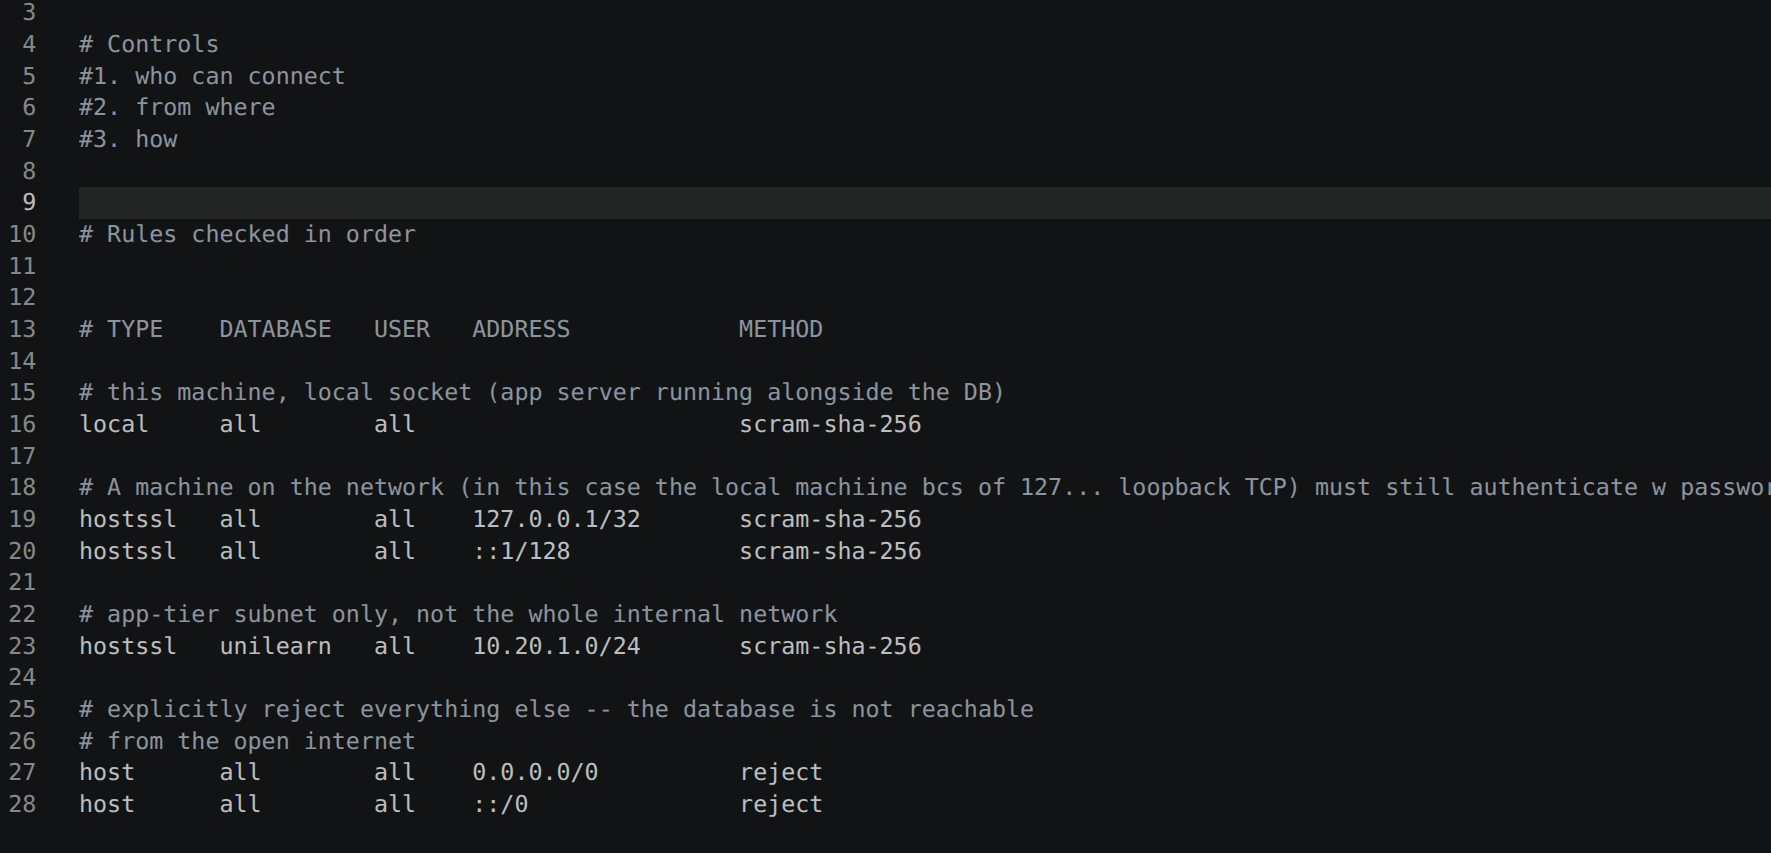
\includegraphics[width=0.85\textwidth]{images/12_pg_hba_conf.png}
\caption{pg\_hba.conf}
\end{figure}

\begin{figure}[H]
\centering
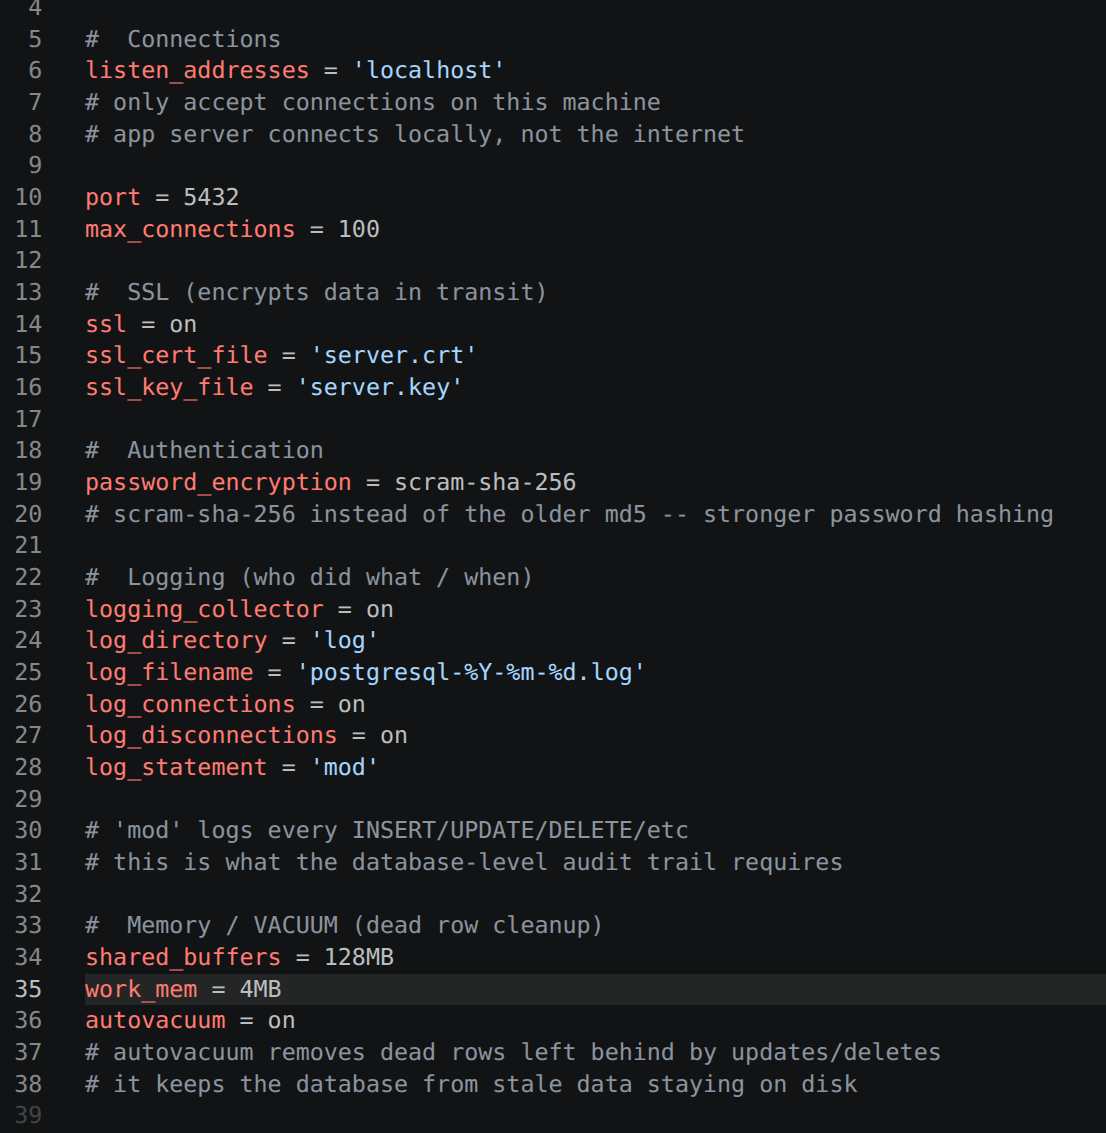
\includegraphics[width=0.75\textwidth]{images/13_postgresql_conf.png}
\caption{postgresql.conf}
\end{figure}

\begin{figure}[H]
\centering
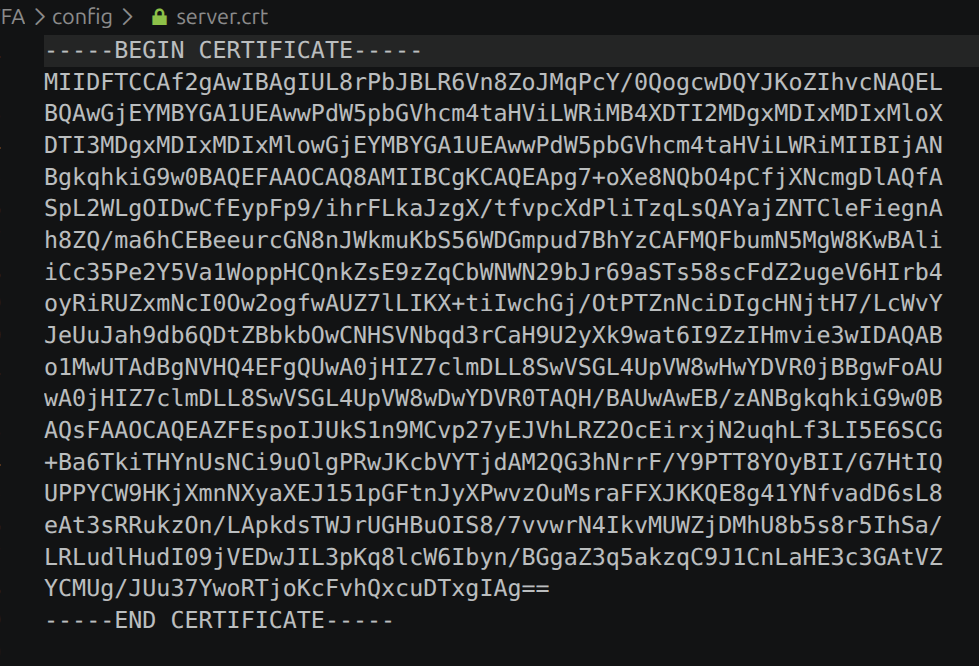
\includegraphics[width=0.55\textwidth]{images/14_server_crt.png}
\caption{server.crt}
\end{figure}

\noindent\textbf{Verification.} I couldn't safely apply this config to the live system PostgreSQL instance directly, it would need root and a full service restart of a shared instance. Instead I built an isolated throwaway PostgreSQL 18 instance in a scratch directory, dropped in the project's actual \lstinline|postgresql.conf|, \lstinline|pg_hba.conf|, \lstinline|server.crt|, and \lstinline|server.key| unmodified, only the port number changed to avoid clashing with the running system instance, and tested it directly.

\footnotesize
\renewcommand{\arraystretch}{1.3}
\begin{longtable}{@{} >{\raggedright\arraybackslash}p{5.5cm} >{\raggedright\arraybackslash}p{9.5cm} @{}}
\caption{Configuration verification against a live instance}\\
\toprule
\textbf{Test} & \textbf{Result} \\
\midrule
\endfirsthead

\toprule
\textbf{Test} & \textbf{Result} \\
\midrule
\endhead

\bottomrule
\endfoot

Plaintext TCP connection (\lstinline|sslmode=disable|) & Rejected. \lstinline|pg_hba.conf rejects connection ... no encryption| \\[0.4em]
SSL TCP connection (\lstinline|sslmode=require|) & Succeeds. \lstinline|TLSv1.3|, \lstinline|TLS_AES_256_GCM_SHA384| \\[0.4em]
Password hash scheme in use & \lstinline|SCRAM-SHA-256|, confirmed via \lstinline|pg_authid| \\[0.4em]
\lstinline|log_statement = mod| & A \lstinline|CREATE TABLE|, \lstinline|INSERT|, \lstinline|DROP TABLE| sequence appeared in the log file verbatim \\

\end{longtable}
\renewcommand{\arraystretch}{1.0}
\normalsize

\newpage
%========================================
\section{SQL Business Logic Executable Script}
\label{sec:task3}
%========================================

\lstinline|business_logic.sh| creates three PL/pgSQL functions against the \lstinline|unilearn| schema, seeds minimal demonstration data, and calls each function to show its behaviour. \lstinline|IM.sql| truncates every table with \lstinline|RESTART IDENTITY CASCADE| without touching structure, so the two scripts together give a repeatable reset and demo cycle. This is what lets the executable be run more than once during marking.

I wrote the script as a \lstinline|.sh| wrapping \lstinline|psql| calls rather than a plain \lstinline|.sql| file, per the brief's requirement that the executable be a shell script, not a SQL dump. Each stage, function creation, seeding, each demo call, is a separate \lstinline|psql| invocation, so the output stays readable as labelled steps rather than one undifferentiated block of results.

\lstinline|IM.sql| uses \lstinline|TRUNCATE ... RESTART IDENTITY CASCADE| rather than \lstinline|DELETE FROM| on each table. \lstinline|TRUNCATE| is faster since it doesn't scan or log individual rows. \lstinline|RESTART IDENTITY| resets every \lstinline|IDENTITY| sequence, so a fresh run produces the same \lstinline|student_id|, \lstinline|enrolment_id|, and so on, as the last one. \lstinline|CASCADE| clears tables in dependency order automatically, rather than me listing 16 tables by hand in an order that respects foreign keys.

\footnotesize
\renewcommand{\arraystretch}{1.3}
\begin{longtable}{@{} >{\raggedright\arraybackslash}p{3.4cm} >{\raggedright\arraybackslash}p{5.8cm} >{\raggedright\arraybackslash}p{5.8cm} @{}}
\caption{Business logic functions}\\
\toprule
\textbf{Function} & \textbf{Behaviour} & \textbf{Why} \\
\midrule
\endfirsthead

\toprule
\textbf{Function} & \textbf{Behaviour} & \textbf{Why} \\
\midrule
\endhead

\bottomrule
\endfoot

\lstinline|fn_enrol_student| & Enrols a student in a course. If already enrolled, raises a notice and returns the existing \lstinline|enrolment_id| instead of erroring & Enrolling twice is a normal user action, a double click or a retry, not an error condition. I treated this as a business logic decision, not a schema one, so it lives in the function rather than relaxing the \lstinline|UNIQUE| constraint \\[0.6em]

\lstinline|fn_course_average| & Returns the average \lstinline|marks_awarded| across a course's graded submissions, or \lstinline|NULL| if nothing is graded yet & Returns \lstinline|NULL|, not \lstinline|0|. An ungraded course is not the same as one averaging zero \\[0.6em]

\lstinline|fn_record_attendance| & Inserts an attendance record. Does nothing on a duplicate, using \lstinline|ON CONFLICT (student_id, schedule_id, attendance_date) DO NOTHING| & Marking the same session twice shouldn't crash a real register \\

\end{longtable}
\renewcommand{\arraystretch}{1.0}
\normalsize

\noindent\textbf{A genuinely interesting result} came from running \lstinline|business_logic.sh| again against a database that still had earlier test data in it, rather than a freshly reset one. The script's raw seed inserts failed loudly and correctly.

\begin{lstlisting}[language=,basicstyle=\ttfamily\footnotesize]
ERROR:  duplicate key value violates unique constraint "departments_department_name_key"
ERROR:  duplicate key value violates unique constraint "roles_role_name_key"
ERROR:  duplicate key value violates unique constraint "programs_program_name_key"
ERROR:  duplicate key value violates unique constraint "staff_email_key"
ERROR:  duplicate key value violates unique constraint "students_email_key"
\end{lstlisting}

But calling \lstinline|fn_enrol_student(1, 1)| a second time against the same already seeded data didn't error. It printed \lstinline|NOTICE: Student 1 already enrolled in course 1 (enrolment_id 1)| and returned the existing row. Same story for \lstinline|fn_record_attendance|. Called twice for the same session, the second call silently did nothing, and \lstinline|SELECT count(*) FROM Attendance| stayed at 1. This is the schema constraint layer and the business logic layer doing their jobs differently on purpose, not a bug. A raw duplicate insert should fail hard, while a function representing a real user action should handle an already done case gracefully. One note for anyone rerunning the demo without a reset in between, \lstinline|Courses|, \lstinline|Schedule|, and \lstinline|Assignments| carry no \lstinline|UNIQUE| constraint on their seed columns, so reseeding against them duplicates rows silently rather than erroring.

The script's own \lstinline|set -e| didn't stop it partway through this, and that is expected, not a flaw. \lstinline|set -e| aborts the bash script if a command exits non zero, but each seeding block is a single \lstinline|psql| invocation reading a whole heredoc of SQL statements. \lstinline|psql|, without \lstinline|ON_ERROR_STOP|, reports each failing statement and moves to the next one within that invocation, then still exits with success once the heredoc is done. That is why the five errors printed rather than killing the script, and why the run still finished with usable output for the rest of the demo.

I confirmed the full cycle was clean. \lstinline|business_logic.sh|, then \lstinline|IM.sql|, then \lstinline|business_logic.sh| again, against a freshly reset database, produced identical output both times with zero errors, including the \lstinline|fn_course_average| calls, which returned \lstinline|NULL| before any grade existed and \lstinline|42.00| immediately after I inserted one, in both runs.

None of the three functions is \lstinline|SECURITY DEFINER|, so each runs with the privileges of whichever role calls it, not the privileges of whoever created it. I tested this directly. \lstinline|student_role| calling \lstinline|fn_enrol_student| for a pair it is already enrolled in works fine, since that path only selects. But \lstinline|student_role| calling it for a genuinely new enrolment fails, with \lstinline|ERROR: permission denied for table enrolments|, because the function's insert runs as \lstinline|student_role|, which only has \lstinline|SELECT| on \lstinline|Enrolments| (Section~\ref{sec:roles}). As written, the enrolment function is only usable end to end by a role with write access to \lstinline|Enrolments|, meaning \lstinline|lecturer_role| or \lstinline|admin_role|, not by the student it is named for. I am flagging this as a real, verified gap between the function's name and what \lstinline|student_role| can actually do with it, rather than leaving it to look like it works for students just because it compiles and runs under a higher privileged role.

\newpage
%========================================
\section{Testing of User Journeys}
\label{sec:testing}
%========================================

\noindent\textbf{A student enrols, is graded, and checks their result.} \lstinline|fn_enrol_student| creates the \lstinline|Enrolments| row. A lecturer later inserts a \lstinline|Submissions| row and a \lstinline|Grades| row against it. The student queries \lstinline|Student_Grade_View| (Section~\ref{sec:roles}) and sees their mark and \lstinline|max_marks|, but not \lstinline|graded_by|. A direct \lstinline|SELECT| on \lstinline|Grades| from the same session is rejected (Section~\ref{sec:verification1}), confirming the view is the only path.

\noindent\textbf{A lecturer records attendance across repeated sessions.} \lstinline|fn_record_attendance| is called once per class. Calling it again for a session already marked does nothing rather than erroring (Section~\ref{sec:task3}), so a resubmitted register can't create duplicate rows or crash the request.

\noindent\textbf{An unauthorised or unencrypted connection is refused before it can do anything.} A plaintext TCP connection is rejected at the connection stage, before authentication runs (Section~\ref{sec:task2}). A \lstinline|read_only_role| session that does connect still cannot write (Section~\ref{sec:verification1}). Network and transport, then privilege, each have to pass independently for a write to happen.

%========================================
\section{Security Design Decisions}
\label{sec:security}
%========================================

Least privilege roles, TLS only remote access with an explicit deny all, SCRAM SHA 256 hashing, and full write and connection audit logging form the core of the design, covered in Sections~\ref{sec:task1} and \ref{sec:task2}. View based column hiding keeps a sensitive column out of a role's reach without per column grants, which PostgreSQL doesn't support directly. I verified every access control decision live under \lstinline|SET ROLE|, not just by reading the grant statements.

\noindent\textbf{Known limitations, not fixed, listed on purpose.}

\begin{enumerate}
    \item No Row Level Security. \lstinline|student_role|'s grant on \lstinline|Student_Grade_View| covers every row, not just that student's own. Enforcing an own rows only rule needs RLS policies, not built yet.
    \item No cross table CHECK on \lstinline|Grades.marks_awarded| against \lstinline|Assignments.max_marks|. This needs a trigger. I left it out to keep the submitted schema simple and fully trigger free.
    \item Self signed SSL certificate. It encrypts the connection but isn't verifiable against a trusted CA.
    \item \lstinline|CREATE ROLE ... PASSWORD 'placeholder_change_me'|. Every role password in \lstinline|schema.sql| is a placeholder, not a real credential.
    \item \lstinline|10.20.1.0/24| in \lstinline|pg_hba.conf| is illustrative, standing in for a segmented app tier subnet. It is not a real deployed address range.
\end{enumerate}

%========================================
\section{AI Use Declaration}
\label{sec:ai}
%========================================

I used AI for the following.

\begin{itemize}
    \item Ran the scripts against a live PostgreSQL instance to check my test claims held up.
    \item Caught a factual error in my privilege test notes, lecturer access to \lstinline|Departments| is read only, not blocked outright.
    \item Formatted the report into LaTeX, matching an example report of mine.
    \item Helped me along with \lstinline|business_logic.sh| and taught me bash as I went, since I had little experience with it. Also helped write the comments.
    \item Debugging help on the isolated PostgreSQL instance used for config verification.
    \item Grammar, punctuation, and phrasing edits, and cut the word count down by rephrasing.
    \item Added the section cross references, and mapped the schema to the GDPR point in the brief.
\end{itemize}

\newpage
%========================================
\section*{Appendix: Full Code Listings}
%========================================

\subsection*{A.1 schema.sql}
\lstinputlisting[language=SQL]{schema.sql}

\subsection*{A.2 business\_logic.sh}
\lstinputlisting[language=bash]{business_logic.sh}

\subsection*{A.3 IM.sql}
\lstinputlisting[language=SQL]{IM.sql}

\subsection*{A.4 config/postgresql.conf}
\lstinputlisting[language=]{config/postgresql.conf}

\subsection*{A.5 config/pg\_hba.conf}
\lstinputlisting[language=]{config/pg_hba.conf}

\subsection*{A.6 config/README.md}
\lstinputlisting[language=]{config/README.md}

\end{document}
